\documentclass[a4paper,10pt]{article}
\usepackage[top=2cm, bottom=2cm, left=2cm, right=2cm]{geometry}
\usepackage[utf8x]{inputenc}
\usepackage[T1]{fontenc}
\usepackage[french]{babel} 
\usepackage{hyperref}
\usepackage{graphicx}
\usepackage{url}
\makeatletter
\g@addto@macro{\UrlBreaks}{\UrlOrds}
\makeatother

\author{\textsc{Awada} Ali, \textsc{Baasandorj} Chinbat \& \textsc{Jorandon} Guillaume}
\date{10 avril 2018} 
\title{Compte rendu d'avancement\\\large{\textit{Industries culturelles et algorithmes de profilage}}\\\normalsize{PH03}}

\begin{document}

\maketitle

Ce document présente brièvement l'état d'avancement du mémoire de PH03.

\section{Présentation}

\subsection{Choix du sujet}

Nous avons choisi pour ce mémoire d'étudier un sujet transverse avec une autre UV de l'UTC, IC01 (Histoire et prospectives des industries culturelles).

Nous sommes partis du constat que le pouvoir des industries culturelles modernes se manifeste de plus en plus au travers de systèmes informatiques de traitement automatique de l'information. En effet, nous sommes désormais à l'ère du Big data, terme souvent détourné à des fins marketing, mais qui renvoie au stockage et à l'analyse de très gros volumes de données. Son utilisation ouvre des perspectives sans commune mesure avec ce que nous aurions eu peine à envisager il y a encore 50 ans.

Le contrôle de ces grands volumes de données donne un pouvoir économique et politique gigantesque aux industries culturelles de masse, comme les GAFAM (Google, Apple, Facebook, Amazon, Microsoft, entreprises américaines majeures dans la collecte de données). Ces nouveaux mastodontes de la culture de masse, organisés en oligopole à frange\footnote{Oligopole où un faible nombre de grosses entreprises domine une majorité du marché, la part restant étant disputée par un grand nombre de petites entreprises. On retrouve cette structure de marché notamment dans les industries culturelles, comme les maisons de disque.}, proposent bien souvent à des consommateurs un large éventail de contenus (produits) culturels : livres (mais pas que, bien sûr) pour Amazon, musique pour Spotify, iTunes, ou films pour Netflix.

Les consommateurs en sont de plus en plus conscients aujourd'hui, mais ces plateformes sont pilotées par des entreprises privées régies bien souvent par le droit américain\footnote{Spotify est une société suédoise cependant.}, avec une politique agressive de collecte des données. Celles-ci peuvent être utilisées pour être revendues à des annonceurs à des fins de publicité ciblée\footnote{Facebook base la quasi intégralité de son modèle économique sur ce modèle.} : il s'agit de contenus commerciaux dont la diffusion a été proposée à telle ou telle personne parce que l'analyse de leurs données a permis de faire un profilage marketing et de dégager de potentielles inclinaisons à la consommation d'un produit donné. 

Mais sans même faire de la publicité, ces plateformes peuvent exploiter les données dans le but de cibler les contenus qu'elles proposent aux consommateurs : Amazon par exemple dispose de plusieurs encarts dédiés aux produits recommandés (exemple figure~\ref{amazon}\footnote{Certaines suggestions (comme \underline{Politiques de l'intimité} de A. \textsc{Mbembe}) font référence à un achat beaucoup plus ancien (\underline{Ruptures postcoloniales}), il y a un an de cela.}).

\begin{figure}[ht]
 \begin{center}
  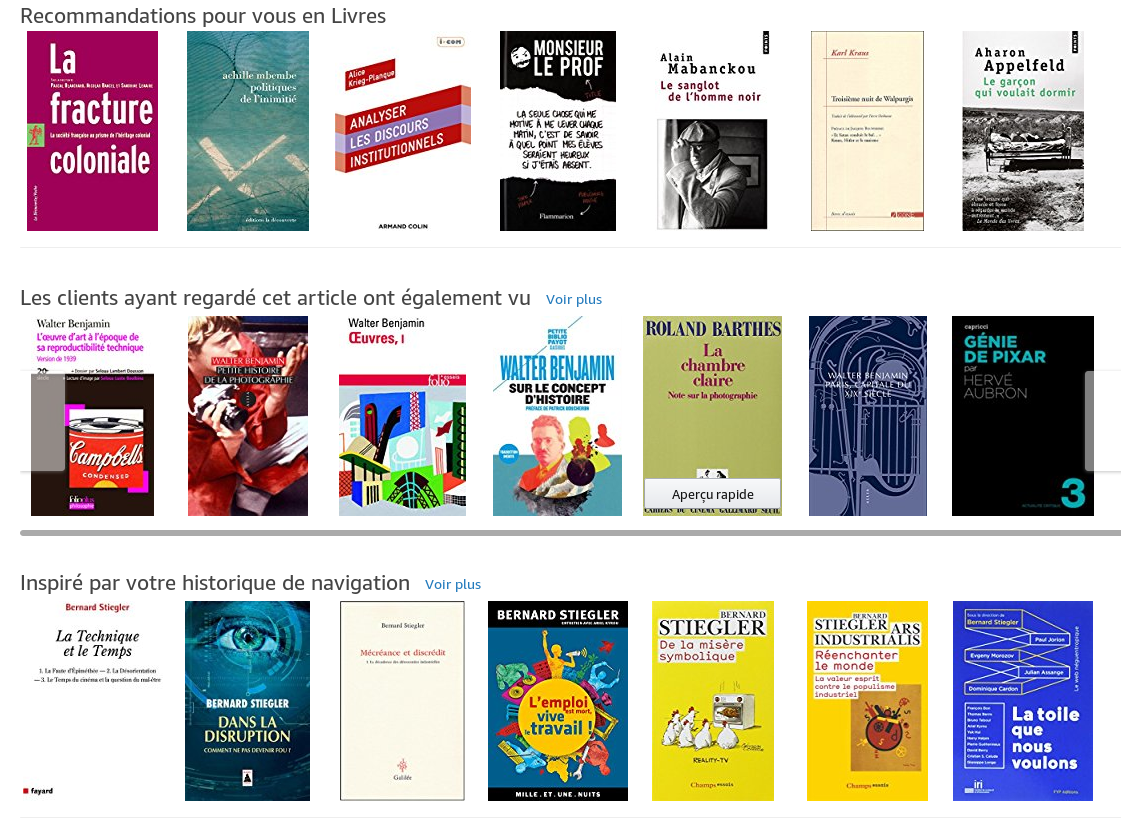
\includegraphics[width=300px]{img/amazon.png}
 \end{center}
		\caption{Quelques jours après avoir commandé plusieurs livres dans le cadre de l'UV PH03, on peut constater l'apparition de nombreuses références en relation avec les livres commandés.}
 \label{amazon}
\end{figure}

Nous pouvons alors légitimement nous demander comment ces plateformes de diffusion de contenu culturel, sur Internet mais aussi dans les médias, à travers les techniques modernes de profilage, façonnent une esthétique fondamentalement politique ? Plus généralement, en quoi ces plateformes, par leur fonctionnement, sont politiques ?

Nous avons choisi de traiter en détail l'une d'entre elles, Netflix, parce qu'elle est une illustration très parlante de ce qu'est une plateforme de diffusion de contenus culturels, mais aussi parce que plusieurs ressources de recherche existent à son sujet.

\subsection{Réflexion sur le plan}

Après avoir délimité le sujet, nous avons mené une réflexion sur le plan, en parallèle de ce que nos premières lectures nous ont permis de constater (voir section~\ref{section_lectures}).

Dans un premier temps, nous nous proposerons de définir clairement ce qu'est une industrie culturelle, et d'étudier leurs évolutions à l'ère du numérique. Nous étudierons ensuite le cas particulier des plateformes de diffusion de contenu et leur utilisation des algorithmes de profilage : comment sélectionnent-ils les contenus, et quels problèmes cela pose-t'il ? Enfin, nous essaierons d'ouvrir le débat en réfléchissant des solutions pour une autre manière de concevoir le décisionnel.

Ce plan n'est pas encore définitif et pourrait évoluer à la lumières de ce que nous avons encore à étudier.

\subsection{Notions abordées}

Nous avons pu dégager quelques notions qui nous semblent pertinentes pour notre étude. Pour chacune d'elles, en voici une brève définition.

\begin{description}
		\item[Industrie culturelle :] entreprises et industries à l'origine des produits culturels de masse : livres, musiques, films, jeux vidéo, etc. Ces biens se caractérisent par le fait que leur valeur intrinsèque est reliée à leur contenu symbolique. Ces entreprises s'inscrivent dans une logique capitaliste productiviste, et est un objet d'étude de l'esthétique (philosophie), mais aussi en sociologie et en sciences de la communication.
		\item[Algorithmes de profilage :] un algorithme au sens large est une séquence d'instructions logiques qui permettent de réaliser une tâche (en ce sens, une recette de cuisine est un algorithme). En informatique, les algorithmes sont le coeur conceptuel des programmes que font tourner nos machines. Les algorithmes de profilage sont des processus informatisés de traitement statistisque de l'information, afin d'extraire d'une masse d'informations brutes des descripteurs signifiants de cette masse de données.
		\item[Prolétarisation :] au sens de Bernard \textsc{Stiegler}, il s'agit de la perte de sens et de savoir. Par exemple, le travail selon \textsc{Stiegler} se prolétarise fortement : les travailleurs ne créent plus de savoir, et les tâches qu'ils exécutent sont de moins en moins contextualisées. On peut penser aux ouvriers d'une chaine de production taylorisée, ou d'un employé de bureau dans les rouages administratifs abscons d'un quelconque service d'une très grande entreprise.
		\item[Néguentropie :] contraire de l'entropie, qui est la dispertion, l'augmentation du désordre. La néguentropie consiste à recréer de l'ordre et du savoir, créer de la valeur ajoutée.
		\item[Big data :] regroupe à la fois les très gros volumes de données, mais aussi leur stockage et leur traitement (data mining). Ces traitements sont essentiellement informatiques, car leur volume même exclue toute possibilité de traitement manuel.
		\item[Philosophie transcendentale (selon Kant) :] concept essentiel de la philosophie moderne, le transcendental désigne les conditions de possibilité. "J'appelle transcendantale toute connaissance qui ne porte point en général sur les objets mais sur notre manière de les connaître, en tant que cela est possible a priori." (Emmanuel Kant \textit{in} \underline{Critique de la raison pure})
\end{description}

\section{État des recherches documentaires}
\label{section_lectures}

Nous allons maintenant résumer l'état d'avancement des recherches documentaires. Nous nous sommes répartis plusieurs lectures qui nous semblaient pertinentes pour notre sujet. Cette section décrit brièvement chaque document visionné/lu ou en cours de lecture/visionnage, pour chacun de nous.

\subsection{Ali \textsc{Awada}}

\subsubsection{\underline{Big data : pour une éthique des données} (Célia \textsc{Zolynski})}

\subsubsection{\underline{Le pouvoir des algorithmes} (Dominique \textsc{Cardon})}

\subsubsection{\underline{L'\oe{}uvre d'art à l'époque de sa reproductibilité} (Walter \textsc{Benjamin})}

\subsection{Chinbat \textsc{Baasandorj}}

\subsubsection{\underline{La technique et le temps, tome 3 : le temps du cinéma et la question du mal-être} (Bernard \textsc{Stiegler})}

\subsubsection{Interview de Bernard Stiegler sur la question de l'art et les industries culturelles}

\subsection{Guillaume \textsc{Jorandon}}

\subsubsection{\underline{Bioestetica, senso comune, tecnica e arte nell'età della globalizzazione} (Pietro \textsc{Montani})}

Pietro \textsc{Montani} (1946-) est un philosophe italien, professeur d'esthétique de l'Université La Sapienza de Rome, et par le passé directeur d'études associées à l'EHESS à Paris. Son oeuvre tourne autour de la philosophie des techniques.

\underline{Bioesthétique} est un essai philosophique sorti en 2007. Il se propose d'étudier comment notre rapport à l'image est en train d'être complètement bouleversé sous l'influence des techniques modernes. Il se propose d'étudier le biopouvoir, c'est à dire un pouvoir centré sur la vie et les corps de la population.

Le livre aborde des notions que nous allons pouvoir réinvestir pour l'étude de notre sujet. Notamment il pose la question des effets de la biopolitique sur les individus. Par exemple, dans le premier chapitre, Montani cite Hannah \textsc{Arendt} (1906-1975), philosophe et politologue d'origine allemande qui s'est spécialisée dans l'étude des totalitarismes et la philosophie de l'Histoire. Dans \underline{La condition de l'homme moderne}, celle-ci expose les prémisses de ce qui va devenir la biopolitique, en postulant que l'humanité moderne, socialisée, ne tourne plus autour de l'Homme ni des hommes, mais autour du processus vital même, autour d'un intérêt de classe ou d'espèce. Il y a disparition de l'intérêt individuel dans les activités. On peut dire que la société se mue en une sorte de rûche ou de fourmilière, centrée autour de la perpétuation de l'espèce. Le but de la vie n'est alors que de travailler et perpétuer sa famille. \textsc{Arendt} fait même le parallèle avec les machines électroniques qui se substituent sans problème à une pensée qui ne se résume plus qu'à un calcul des conséquences. On voit alors comment  la notion de biopolitique va nous aider dans notre étude, en utilisant ce prisme d'analyse pour comprendre comment les industries culturelles peuvent exercer une forme de pouvoir sur les individus.

La lecture du texte n'est cependant pas encore terminée, et ce n'est pas un livre facile, car il semble tout de même s'adresser à des lecteurs aguerris. Cependant, nous avons pu constater qu'il avait des références communes aux autres auteurs : \textsc{Kant}, \textsc{Husserl}, \textsc{Heidegger}, \textsc{Adorno}...

\subsubsection{Cours d'IC01}

On peut constater dans nos recherches qu'un nom revient assez souvent : Bernard \textsc{Stiegler}. Il enseigne en effet l'UV IC01 à l'UTC, UV d'où est partie la réflexion sur la construction du sujet, et les industries culturelles sont le fer de lance de ses recherches. Le cours d'IC01, (que je suis actuellement) explique de nombreuses notions que nous pouvons réinvestir dans notre étude.

Par ailleurs, un exposé que j'ai fait dans le cadre de cette UV parle justement de l'émergence de la publicité ciblée dans l'après guerre, à travers l'analyse de \underline{La persuasion clandestine} de Vance \textsc{Packard}.

\subsubsection{Langues de bois épisode 10 : "Les français veulent que..." (Le Stagirite)}

Le Stagirite (de son vrai nom Fabrice) est un vidéaste qui parle de l'utilisation des procédés rhétoriques en politique. Dans cette vidéo, traitant de l'utilisation des sondages en politique en France, il explique que les sondages d'opinion échouent à proposer un baromètre de l'opinion publique, parce que cette opinion publique n'existe pas (Pierre \textsc{Bourdieu}). Au lieu de cela, les sondages mesurent en réalité l'opinion des gens sur les opinions des décideurs politiques, dans des termes déjà posés a priori. Cette idée que les procédés de fabrication de l'opinion se font autour de termes déjà posés à l'avance pourrait se creuser dans notre sujet : est-ce que les algorithmes de profilages ne contribuent-ils pas à créer une esthétique politique sur la base de termes déjà existants ?

Le pouvoir a les moyens de faire advenir l'état de l'opinion qu'elle postule. Il ne s'exerce pas directement, mais indirectement en cadrant le débat, et en imposant des problématiques. En ce sens on peut trouver dans les propos de la vidéo l'illustration d'une forme de biopouvoir. Le Stagirite évoque d'ailleurs l'idée d'un marché de l'idéologie politique, où les opinions sont mises en concurrence. Dans notre cas, on pourrait considérer que les agents de ce marché ne sont pas des politiciens, mais des systèmes décisionnels informatisés.

\subsubsection{\underline{Les nouveaux chiens de garde} (Serge \textsc{Halimi}) et \underline{La fabrication du consentement} (Noam \textsc{Chomsky})}

\underline{Les nouveaux chiens de garde} est un essai du journaliste Serge \textsc{Halimi} (1955-), que j'ai lu l'année dernière. Rédigé dans un style plus journalistique, \textsc{Halimi} expose comment l'opinion est prescrite par une caste médiatique, en étroite relation avec le monde politico-politicien : il s'attache ainsi à comprendre les connivences qui existent au sein du marché de l'information. Même si ce texte est apparemment sans rapport avec notre sujet, on peut y trouver certains apports utiles, notamment la manière qu'a \textsc{Halimi} de considérer l'information comme une marchandise comme une autre. 

Dans le même ordre d'idées, \underline{La fabrication du consentement} est un essai (que j'ai aussi lu l'année dernière) de Noam \textsc{Chomsky} (1928-), linguiste américain majeur du 20\textsuperscript{e} siècle, bien que très controversé. Dans ce livre, \textsc{Chomsky} étudie lui aussi comment se construit l'opinion au sein de la démocratie médiatique américaine. Cet auteur est cependant sujet à caution, et certains de ses contemporains (comme Bernard \textsc{Stiegler}), lui reprochent un dédain injustifié de la philosophie européenne : \textsc{Chomsky} a battu en brèche la psychanalyse, notamment Lacanienne, et plus globalement toute la French Theory, qui regroupe plusieurs penseurs du relativisme postmoderne, comme \textsc{Deleuze}, \textsc{Foucault} ou \textsc{Derrida}. Jusqu'au-boutiste, il a aussi été au coeur de la polémique lors de l'affaire \textsc{Faurisson}, en prenant la défense par principe de Robert Faurisson, négationniste convaincu, au nom de la liberté d'expression.

Une notion se retrouve dans les deux essais, et qu'il va être important de prendre en compte pour la suite de notre étude, est que pour comprendre les jeux de pouvoir et d'influence, il n'est nul besoin de faire appel à la théorie du complot, là où l'étude des structures et des contraintes suffit. En effet, il aurait été facile pour \textsc{Halimi} et \textsc{Chomsky} d'affirmer que si les médias influencent l'opinion, c'est forcément parce que les agents sont corrompus, payés, ou complotent dans l'ombre pour manipuler activement la population, dans une caricature du complot illuminati ou reptilien. De même, il serait facile pour nous de faire ce genre d'affirmation pour expliquer les motivations profondes qui poussent les plateformes de diffusion culturelles à pister et influencer leurs consommateurs. Or, une théorie du complot est une hypothèse très couteuse et qui soulève bien plus de questions qu'elle n'en résout. Nous devrons donc, pour notre étude, nous prémunir de ce genre d'argumentation. Ce principe de raisonnement, qui consiste à écarter les hypothèses épistémologiquement couteuses, porte un nom : le rasoir d'Ockham.

\section{Travaux restants}

Pour la suite du semestre, nous allons continuer et terminer nos lectures actuelles. Une fois cela fait, il pourrait être utile d'approfondir un peu certains auteurs qui reviennent d'un texte à l'autre (\textsc{Kant}, \textsc{Adorno}...).

Nous devrons ensuite étudier en détail le cas Netflix pour trouver des réponses à notre problématique. Nous réflechissons par ailleurs à interviewer un acteur du milieu, Bernard \textsc{Stiegler} ou autre, pour des questions plus pointues.

\end{document}
